\subsection{Vertex Reconstruction}\label{section:star_vertex}

In $pp$ collisions, where the charged-particle multiplicity is low, the vertex finding algorithm sometimes fails to find a primary vertex. In addition, at high luminosity, vertex finder can fail due to the contribution of pile-up events and providing a wrong reconstructed vertex. In this study we required at least two reconstructed global tracks $n^{global}_{sel}\geq 2$ passing all the quality cuts listed in Sec~\ref{section:star_track_selection} but without $DCA_{xy}$ and $DCA_{z}$ cuts.  Additionally, MC events were accepted if a $z$-coordinate of the true-level primary vertex was between $-80$ and $80$~cm. All corrections, described in this section, were calculated in three ranges of $\xi$ separately.

\subsubsection{Track quality cuts used for vertexing}
The following quality cuts had to be passed by the global tracks used in the vertex reconstruction:
\begin{enumerate}
	\item Tracks must be matched with hits reconstructed in TOF,
	\item The number of the TPC hits used in the helix fit $N_{hits}^{fit}$ must be greater than 20,
	\item The ratio of the number of TPC hits used in the helix fit to the number of possible TPC hits $N_{hits}^{fit}/N_{hits}^{poss}$ must be greater than $0.52$,
	\item The transverse impact parameter with respect to the beamline $d_0$ must be less than 2 cm,
	\item The track's transverse momentum $p_T$ must be greater than $0.2$~GeV/c.
\end{enumerate}
 Above track selection criteria are different than those used in the analysis. Since that, primary vertex reconstruction efficiency and fake vertex rate were calculated as a function of number of global tracks used in vertexing $n^{global}_{vrt}$ instead of $n^{global}_{sel}$. 

\subsubsection{Vertex efficiency and fake vertex rate}
In every MC event there is a well defined primary vertex.  With the embedded event reconstructed and the MC information in hand,
the vertex-finding efficiency can be obtained. In the analysis exactly one single TOF vertex with $n_{sel}\geq 2$ is required.  The reconstructed vertex with the label \textit{best} is the one with the highest number of TOF-matched tracks. Since the fake vertices (not matched to the true-level primary vertex) were allowed in the analysis, the overall vertex-finding efficiency, $\epsilon_{vrt}\left(n_{vrt}^{global}\right)$, is expressed as:

\begin{equation}
\epsilon_{vrt}\left(n_{vrt}^{global}\right)=\epsilon_{vrt}^ {best}\left(n_{vrt}^{global}\right)+\delta_{vrt}^{fake}\left(n_{vrt}^{global}\right)
\end{equation}
where:
\begin{description}
	\item $\epsilon_{vrt}^ {best}\left(n_{vrt}^{global}\right)$ is the primary vertex reconstruction efficiency, determined as the ratio of the number of good reconstructed events (reconstructed best primary vertex with $n_{sel}\geq 2$) to the number of input MC events, where the reconstructed vertex is matched to the true-level primary vertex,
	\item $\delta_{vrt}^{fake}\left(n_{vrt}^{global}\right)$ is the fake vertex rate, determined as the ratio of the number of good reconstructed events (reconstructed best primary vertex with $n_{sel}\geq 2$) to the number of input MC events, where the reconstructed vertex is not matched to the true-level primary vertex.
\end{description}

The vertex-finding efficiency as a function of $n^{global}_{vrt}$ is shown in  Fig.~\ref{fig:vertexEffi}~(left). When there are exactly two global tracks used in the vertex reconstruction, $n^{global}_{vrt}=2$, the longitudinal distance between these tracks $|\Delta z_0|$  is utilized by the vertex-finding algorithm. Since that, the vertex finding efficiency for such events $\epsilon_{vrt}\left(|\Delta z_0|\right)$ is given by:
\begin{equation}
\epsilon_{vrt}\left(|\Delta z_0|\right)=\epsilon_{vrt}^ {best}\left(|\Delta z_0|\right)+\delta_{vrt}^{fake}\left(|\Delta z_0|\right)
\end{equation}
where:
\begin{description}
	\item $\epsilon_{vrt}^ {best}\left(|\Delta z_0|\right)$ is the primary vertex reconstruction efficiency,
	\item $\delta_{vrt}^{fake}\left(|\Delta z_0|\right)$ is the fake vertex rate.
\end{description}
Figure~\ref{fig:vertexEffi}~(right) shows the vertex finding efficiency for events with $n^{global}_{vrt}=2$. This efficiency is smaller than $20\%$ for tracks with $|\Delta z_0|>2$~cm, hence the analysis was limited to  events with  $|\Delta z_0|<2$~cm, when $n^{global}_{vrt}=2$. 
\begin{figure}[h!]
	\centering
		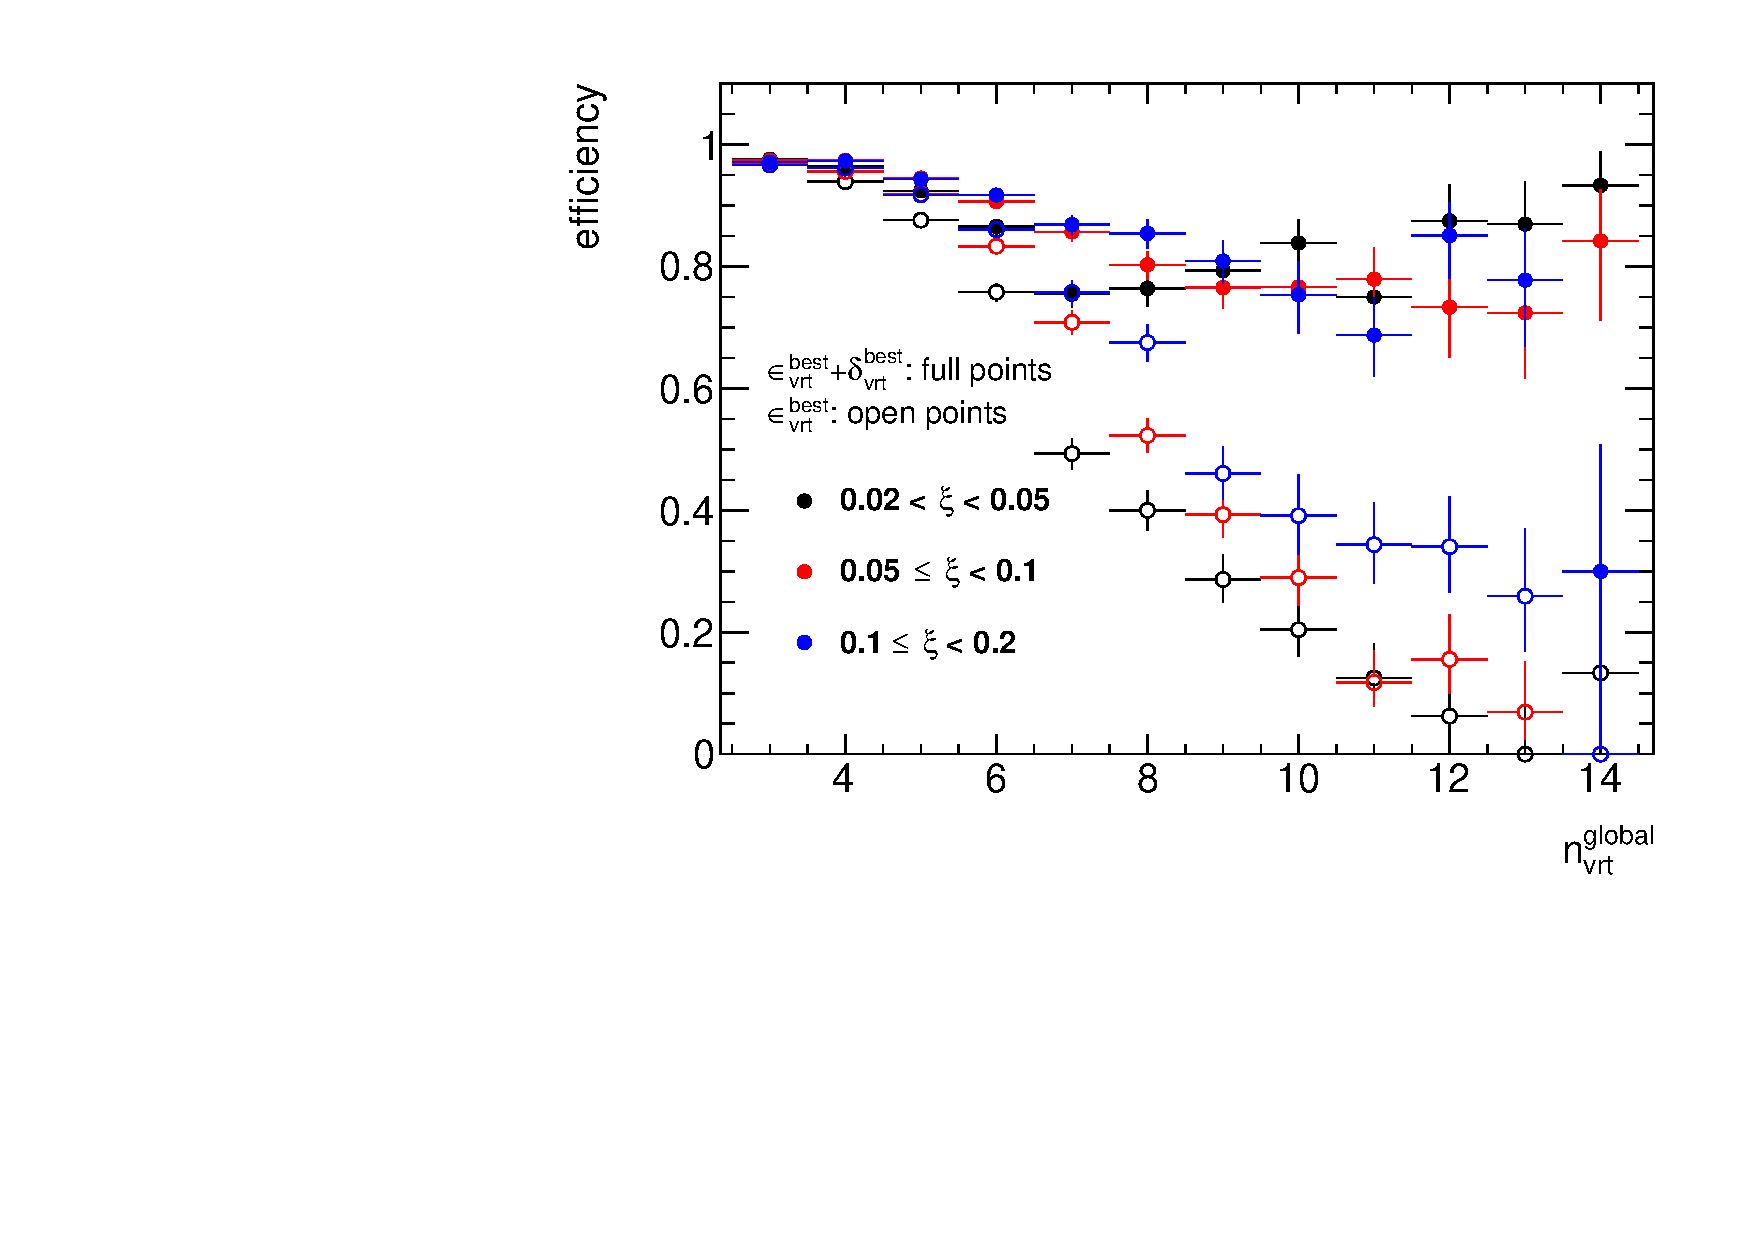
\includegraphics[width=0.49\textwidth,page=1]{chapters/chrgSTAR/img/vertex/vertexEffi_ksi.pdf}
		\includegraphics[width=0.49\textwidth,page=8]{chapters/chrgSTAR/img/vertex/vertexEffi_ksi.pdf}
		\caption[Vertex-finding efficiency in three ranges of $\xi$ as a function of $n^{global}_{vrt}$ and with respect to the $|\Delta z_0|$ between reconstructed tracks in events with $n^{global}_{vrt}=2$]{Vertex-finding efficiency in three ranges of $\xi$ as a function of $n^{global}_{vrt}$ (left) and with respect to the $|\Delta z_0|$ between reconstructed tracks in events with $n^{global}_{vrt}=2$ (right). }
		\label{fig:vertexEffi}
\end{figure}

\subsubsection{Other corrections to the reconstructed vertices}
Events with reconstruced best vertex are rejected if there  are:
\begin{enumerate}[label=\alph*)]
	\item more than one additional TOF vertices,
	\item additional secondary TOF vertex from the interactions with the detector dead-material,
	\item additional fake TOF vertex,
	\item additional primary TOF vertex (vertex splitting or background vertex reconstructed as best vertex),
	\item additional decay TOF vertex.  
\end{enumerate}
The correction for vetoing such events, $\epsilon_{vrt}^{veto}\left(n_{vrt}^{global}\right)$, is given by: 
\begin{equation}
\begin{split}
\epsilon_{vrt}^{veto}\left(n_{vrt}^{global}\right) & =1-\frac{\textrm{number of events with more than one reconstructed  TOF vertex}}{\textrm{number of events with at least one reconstructed TOF vertex}} \\
& =1-a-b-c-d-e
\end{split}
\end{equation}
where $a-e$ are the fractions of events with additional vertices, whose labels  are listed above.% shown in \ref{fig:vertexVeto}.

As before, the correction was calculated as a function of $|\Delta z_0|$ for events with $n^{global}_{vrt}=2$. Figure~ \ref{fig:vertexVeto} shows the fraction of multi-vertex events  with respect to the $n_{vrt}^{global}$, where each contribution is shown separately. The analysis was limited to events with $n_{sel}\leq8$, because the $\epsilon_{vrt}^{veto}(n_{vrt}^{global})$ is small ( $<50\%$) above that limit. On the other hand,  the total fraction of multi-vertex events, $a+b+c+d+e$, as a function of $|\Delta z_0|$, shown in Fig.~\ref{fig:vertexVetoDZ}, demonstrates that $\epsilon_{vrt}^{veto}(|\Delta z_0|)$ is very large ($>98\%$) for events with $n^{global}_{vrt}=2$ .
\captionsetup{format=plain,indention=0pt,justification=justified}
\begin{figure}[h!]
	\centering
	\begin{subfigure}{.49\textwidth}
		\includegraphics[width=\textwidth,page=3]{chapters/chrgSTAR/img/vertex/vertexEffi_ksi.pdf}
	\end{subfigure}
	\begin{subfigure}{.49\textwidth}
		\includegraphics[width=\textwidth,page=4]{chapters/chrgSTAR/img/vertex/vertexEffi_ksi.pdf}
	\end{subfigure}
	\begin{subfigure}{.49\textwidth}
		\includegraphics[width=\textwidth,page=5]{chapters/chrgSTAR/img/vertex/vertexEffi_ksi.pdf}
	\end{subfigure}
	\begin{subfigure}{.49\textwidth}
		\includegraphics[width=\textwidth,page=6]{chapters/chrgSTAR/img/vertex/vertexEffi_ksi.pdf}
	\end{subfigure}
	\begin{subfigure}{.49\textwidth}
		\includegraphics[width=\textwidth,page=7]{chapters/chrgSTAR/img/vertex/vertexEffi_ksi.pdf}
	\end{subfigure}
	\begin{minipage}{.49\textwidth}
			\caption[Fraction of multi-vertex events  with respect to the $n_{vrt}^{global}$ in three ranges of $\xi$.]{Fraction of multi-vertex events  with respect to the $n_{vrt}^{global}$ in three ranges of $\xi$. Each contribution is shown separately: more than one additional vertices (top left), additional secondary vertex from the interactions with the detector dead-material (top right), additional fake vertex (middle left), additional primary vertex (middle right) and additional decay vertex (bottom).}
			\label{fig:vertexVeto}
	\end{minipage}

\end{figure}

\begin{figure}[h!]
	\centering
	\begin{subfigure}{.49\textwidth}
		\includegraphics[width=\textwidth,page=9]{chapters/chrgSTAR/img/vertex/vertexEffi_ksi.pdf}
	\end{subfigure}
	\begin{minipage}{.49\textwidth}
		\caption{Total fraction of multi-vertex events as a function of $|\Delta z_0|$ for events with $n^{global}_{vrt}=2$  in three ranges of $\xi$.}
		\label{fig:vertexVetoDZ}
	\end{minipage}
\end{figure}
\captionsetup{format=default,indention=0pt,justification=justified}
\FloatBarrier